\section*{BÀI TẬP PTLGCB}
\setcounter{ex}{0}\setcounter{bt}{0}
\Opensolutionfile{ans}[ans/ansBTTeX1]

\begin{ex}%[1K1Y4-3]%[Chuyên đề Toán 11 - 2023]%[Dương Phước Sang, dự án WTB - Toán 11 - new 2023]
Phương trình lượng giác $3\cot x-\sqrt{3}=0$ có nghiệm là
\choice
{$x=\dfrac{\pi}{3}+k2\pi$}
{Vô nghiệm}
{$x=\dfrac{\pi}{6}+k\pi$}
{\True $x=\dfrac{\pi}{3}+k\pi$}
\loigiai{
Ta có $3\cot x-\sqrt{3}=0 \Leftrightarrow \cot x=\dfrac{\sqrt{3}}{3} \Leftrightarrow \cot x=\cot \left( \dfrac{\pi}{3} \right) \Leftrightarrow x=\dfrac{\pi}{3}+k\pi$, $\left( k \in \mathbb{Z} \right)$.
}
\end{ex}


\begin{ex}%[Thành Đức Trung, Hàm số - Đợt 2 - Tư duy mở]%[1K1B4-9]
Giá trị nhỏ nhất của hàm số $y = \dfrac{\cos^2x + \sin2x}{2\sin^2x + 2\cos2x+2}$ bằng
\choice
{$-\dfrac{1}{2}$}
{\True $-\dfrac{1}{4}$}
{$-1$}
{$0$}
\loigiai
{
Tập xác định $\mathscr{D}=\mathbb{R}$. \\
Ta có
\[\begin{aligned}
y = \dfrac{\cos^2x + \sin2x}{2\sin^2x + 2\cos2x+2}&\Leftrightarrow y=\dfrac{\dfrac{1+\cos2x}{2} + \sin 2x}{2\cdot\dfrac{1-\cos2x}{2} + 2\cos 2x+2} \\
&\Leftrightarrow y = \dfrac{1+\cos2x + 2\sin 2x}{6 + 2\cos2x}\\
&\Leftrightarrow y\left(6 + 2\cos2x\right) = 1 + \cos 2x + 2\sin 2x\\
&\Leftrightarrow (2y - 1)\cos 2x - 2\sin 2x = 1-6y.
\end{aligned}\]
Điều kiện để phương trình trên có nghiệm là
\[(2y - 1)^2 + (-2)^2\ge (1-6y)^2 \Leftrightarrow 32y^2 - 8y - 4 \le 0 \Leftrightarrow -\dfrac{1}{4}\le y\le \dfrac{1}{2}.\]
Vậy $\min\limits_{\mathbb{R}} y=-\dfrac{1}{4}$.
}
\end{ex}

\begin{ex}%[1K1B4-3]
Phương trình $\sin\left(2x-\dfrac{\pi}{3}\right)=0$ có nghiệm là
\choice
{$x=k\pi ,\,k\in\mathbb{Z}$}
{\True $x=\dfrac{\pi}{6}+\dfrac{k\pi}{2},\,k\in\mathbb{Z}$}
{$x=\dfrac{\pi}{2}+k\pi ,\,k\in\mathbb{Z}$}
{$x=\dfrac{\pi}{3}+k\pi ,\,k\in\mathbb{Z}$}
\loigiai{
Ta có $\sin\left(2x-\dfrac{\pi}{3}\right)=0\Leftrightarrow $ $ 2x-\dfrac{\pi}{3}=k\pi ,\,k\in\mathbb{Z}$\\
$\Leftrightarrow x=\dfrac{\pi}{6}+\dfrac{k\pi}{2},\,k\in\mathbb{Z}$.}
\end{ex}

\begin{ex}%[1K1B4-3]
Nghiệm của phương trình $ 3\sin\left(4x+\dfrac{1}{2}\right)-1=0$ là
\choice
{$\left[\begin{aligned}
& x=\dfrac{1}{8}-\dfrac{1}{4}\arcsin\dfrac{1}{3}+k\dfrac{\pi}{2}\\
& x=\dfrac{\pi}{4}-\dfrac{1}{8}-\dfrac{1}{4}\arcsin\dfrac{1}{3}+k\dfrac{\pi}{2}\\
\end{aligned}\right.,k\in\mathbb{Z}$}
{$\left[\begin{aligned}
& x=-\dfrac{1}{8}-\dfrac{1}{4}\arcsin\dfrac{1}{3}+k\dfrac{\pi}{2}\\
& x=\dfrac{\pi}{4}-\dfrac{1}{4}\arcsin\dfrac{1}{3}+k\dfrac{\pi}{2}\\
\end{aligned}\right.,k\in\mathbb{Z}$}
{$\left[\begin{aligned}
& x=-\dfrac{1}{8}+k\dfrac{\pi}{2}\\
& x=\dfrac{\pi}{4}+k\dfrac{\pi}{2}\\
\end{aligned}\right.,k\in\mathbb{Z}$}
{\True $\left[\begin{aligned}
& x=-\dfrac{1}{8}+\dfrac{1}{4}\arcsin\dfrac{1}{3}+k\dfrac{\pi}{2}\\
& x=\dfrac{\pi}{4}-\dfrac{1}{8}-\dfrac{1}{4}\arcsin\dfrac{1}{3}+k\dfrac{\pi}{2}\\
\end{aligned}\right.,k\in\mathbb{Z}$}
\loigiai{
$ 3\sin\left(4x+\dfrac{1}{2}\right)-1=0\Leftrightarrow\sin\left(4x+\dfrac{1}{2}\right)=\dfrac{1}{3}\Leftrightarrow\left[\begin{aligned}
& 4x+\dfrac{1}{2}=\arcsin\dfrac{1}{3}+2k\pi\\
& 4x+\dfrac{1}{2}=\pi-\arcsin\dfrac{1}{3}+2k\pi\\
\end{aligned}\right.,k\in\mathbb{Z}$\\
$\Leftrightarrow\left[\begin{aligned}
& x=-\dfrac{1}{8}+\dfrac{1}{4}\arcsin\dfrac{1}{3}+k\dfrac{\pi}{2}\\
& x=\dfrac{\pi}{4}-\dfrac{1}{8}-\dfrac{1}{4}\arcsin\dfrac{1}{3}+k\dfrac{\pi}{2}\\
\end{aligned}\right.,k\in\mathbb{Z}$}
\end{ex}

\begin{ex}%[1K1B4-3]
Nghiệm của phương trình $2\sin x+1=0$ được biểu diễn trên đường tròn lượng giác trong hình dưới đây là những điểm nào?
\begin{center}
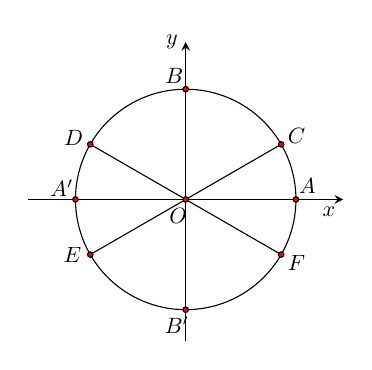
\begin{tikzpicture}[>=stealth,every node/.style={scale=0.8}]
\def\a{1.4}
\path
(0,0)coordinate (O)
(0:\a) coordinate (A)
(180:\a) coordinate (A')
(90:\a) coordinate (B)
(-90:\a) coordinate (B')
(30:\a) coordinate (C)
(150:\a) coordinate (D)
(210:\a) coordinate (E)
(-30:\a) coordinate (F);
\draw (O) circle (\a);
\draw[->] (-2,0)--(2,0)node[below left]{$x$};
\draw[->] (0,-1.8)--(0,2)node[left]{$y$};
\draw (E)--(C) (D)--(F);
\foreach \t/\g in {O/245,A/50,A'/140,B/130,B'/-120,C/30,E/180,D/160,F/-30}{\draw[fill=red,draw=black] (\t) circle (1pt) node[shift={(\g:8pt)}]{$\t$};
}
\end{tikzpicture}
\end{center}
\choice
{Điểm $D$, điểm $C$}
{\True Điểm $E$, điểm $F$}
{Điểm $C$, điểm $F$}
{Điểm $E$, điểm $D$}
\loigiai{
Ta có $2\sin x+1=0\Leftrightarrow \sin x=-\dfrac{1}{2}\Leftrightarrow \hoac{& x=-\dfrac{\pi}{6}+k2\pi \quad (*) \\
& x=\dfrac{7\pi }{6}+k2\pi \quad (**)} \quad (k\in \mathbb{Z}).$\\
Ta có điểm biểu diễn của họ nghiệm $(*)$ là điểm $F$, điểm biểu diễn của họ nghiệm $(**)$  là điểm $E$.}
\end{ex}

\begin{ex}%[1K1B4-3]
Phương trình $\cos x=-\dfrac{\sqrt{3}}{2}$ có tập nghiệm là
\choice
{$\left\{ x=\pm \dfrac{\pi}{3}+k\pi; k\in \mathbb{Z} \right\}$}
{$\left\{ x=\pm \dfrac{\pi}{6}+k\pi; k\in \mathbb{Z} \right\}$}
{\True $\left\{ x=\pm \dfrac{5\pi }{6}+k2\pi; k\in \mathbb{Z} \right\}$}
{$\left\{ x=\pm \dfrac{\pi}{3}+k2\pi; k\in \mathbb{Z} \right\}$}
\loigiai{
$\cos x=-\dfrac{\sqrt{3}}{2}\Leftrightarrow \cos x=\cos \left( \dfrac{5\pi }{6} \right)\Leftrightarrow x=\pm \dfrac{5\pi }{6}+k2\pi \quad (k\in \mathbb{Z})$.}
\end{ex}

\begin{ex}%[1K1B4-3]%[Chuyên đề Toán 11 - 2023]%[Dương Phước Sang, dự án WTB - Toán 11 - new 2023]
Số điểm biểu diễn nghiệm của phương trình $\tan 2x=1$ trên đường tròn lượng giác là
\choice
{$6$}
{$2$}
{$8$}
{\True $4$}
\loigiai{
Ta có $\tan 2x=1 \Leftrightarrow 2x=\dfrac{\pi}{4}+k\pi \Leftrightarrow x=\dfrac{\pi}{8}+\dfrac{k2\pi}{4}$ $\left( k \in \mathbb{Z} \right)$.\\
Vậy số điểm biểu diễn nghiệm của phương trình $\tan 2x=1$ là $4$.
}
\end{ex}

\begin{ex}%[Chuyên đề Toán 11 - 2023]%[Quan Ón, dự án WTB - Toán 11 - new 2023]%[1K1B4-5]
Phương trình $\sin \left( x+\dfrac{\pi}{4} \right)+\cos x=0$ có tập nghiệm được biểu diễn bởi bao nhiêu điểm trên đường tròn lượng giác?
\choice
{$1$}
{\True $2$}
{$4$}
{$3$}
\loigiai{
Ta có
\[\sin \left( x+\dfrac{\pi}{4} \right)+\cos x = 0 \Leftrightarrow \sin \left( x+\dfrac{\pi}{4} \right) = \sin \left( x-\dfrac{\pi}{2} \right) \Leftrightarrow \hoac{&x + \dfrac{\pi}{4} = x - \dfrac{\pi}{2}+k2\pi\\&x+\dfrac{\pi}{4} = \pi - x+\dfrac{\pi}{2}+k2\pi} \Leftrightarrow 2x = \dfrac{5\pi}{4}+k2\pi \Leftrightarrow x=\dfrac{5\pi}{8}+k\pi, \,\, k \in \mathbb{Z}.\]
Cung $x = \dfrac{5\pi}{8} + k\pi$, $k \in \mathbb{Z}$ biểu diễn được hai điểm trên đường tròn lương giác.
}
\end{ex}

\begin{ex}%[1K1B4-3]
Phương trình $\sin\left(x-\dfrac{\pi}{3}\right)=1$ có nghiệm là
\choice
{$ x=\dfrac{\pi}{3}+k2\pi $}
{$ x=\dfrac{5\pi}{6}+k\pi $}
{\True $ x=\dfrac{5\pi}{6}+k2\pi $}
{$ x=\dfrac{\pi}{3}+2\pi $}
\loigiai{
$\sin\left(x-\dfrac{\pi}{3}\right)=1$$\Leftrightarrow x-\dfrac{\pi}{3}=\dfrac{\pi}{2}+k2\pi $ $\Leftrightarrow x=\dfrac{5\pi}{6}+k2\pi $ $\left(k\in\mathbb{Z}\right)$.}
\end{ex}

\begin{ex}%[Chuyên đề Toán 11 - 2023]%[Quan Ón, dự án WTB - Toán 11 - new 2023]%[1K1B4-5]
Tìm số nghiệm của phương trình $\sin \left( \cos 2x \right)=0$ trên $\left[ 0;2\pi \right]$.
\choice
{$2$}
{$1$}
{\True $4$}
{$3$}
\loigiai{
Ta có $\sin (\cos 2x)=0 \Leftrightarrow \cos 2x=k\pi$ $\left( k \in \mathbb{Z} \right)$.\\
Vì $\cos 2x \in [-1;1] \Rightarrow k=0 \Rightarrow \cos 2x=0 \Leftrightarrow 2x=\dfrac{\pi}{2}+k_1\pi \Leftrightarrow x=\dfrac{\pi}{4}+k_1\dfrac{\pi}{2} $ $\left( k_1 \in \mathbb{Z} \right)$.\\
Mà $x \in \left[ 0;2\pi \right] \Rightarrow k_1 \in \big\{0;1;2;3\big\}$.\\
Vậy phương trình đã cho có $4$ nghiệm trên $\left[ 0;2\pi \right]$.
}
\end{ex}

\begin{ex}%[1K1B4-3]
Số nghiệm phương trình $\dfrac{\sin 3x}{\cos x+1}=0$ thuộc đoạn $\left[2\pi ;4\pi\right]$ là
\choice
{$ 7$}
{\True $ 6$}
{$ 4$}
{$ 5$}
\loigiai{
Điều kiện: $\cos x+1\ne 0\Leftrightarrow x\ne\pi+k2\pi $ .\\
Ta có $\dfrac{\sin 3x}{\cos x+1}=0\Rightarrow\sin 3x=0\Leftrightarrow x=\dfrac{k\pi}{3}\left(k\in\mathbb{Z}\right).$\\
So với điều kiện nghiệm của phương trình là $ x=\dfrac{k\pi}{3}$ với $ k\in\mathbb{Z},\,\,k\ne 3\left(2l+1\right)$\\
Vì $ 2\pi\le x\le 4\pi\Leftrightarrow 2\pi\le\dfrac{k\pi}{3}\le 4\pi\Leftrightarrow 6\le k\le 12$ nên ta chọn $ k\in\left\{ 6,7,8,10,11,12\right\}$.}
\end{ex}

\begin{ex}%[Chuyên đề Toán 11 - 2023]%[Quan Ón, dự án WTB - Toán 11 - new 2023]%[1K1B4-3]
Giải phương trình $\left( 2\cos \dfrac{x}{2}-1 \right)\left( \sin \dfrac{x}{2}+2 \right)=0$
\choice
{$x = \pm \dfrac{2\pi}{3}+k2\pi$, $\left( k \in \mathbb{Z} \right)$}
{$x = \pm \dfrac{\pi}{3}+k2\pi$, $\left( k \in \mathbb{Z} \right)$}
{$x = \pm \dfrac{\pi}{3}+k4\pi$, $\left( k \in \mathbb{Z} \right)$}
{\True $x = \pm \dfrac{2\pi}{3}+k4\pi$, $\left( k \in \mathbb{Z} \right)$}
\loigiai{
Vì $-1 \leq \sin \dfrac{x}{2} \leq 1,\,\forall x \in \mathbb{R} \Rightarrow \sin \dfrac{x}{2} + 2 > 0$.\\
Do đó, phương trình đã cho tương đương
\[2\cos \dfrac{x}{2}-1 = 0 \Leftrightarrow \cos \dfrac{x}{2}=\dfrac{1}{2} \Leftrightarrow \dfrac{x}{2}=\pm \dfrac{\pi}{3}+k2\pi \Leftrightarrow x=\pm \dfrac{2\pi}{3}+k4\pi, \, \left( k \in \mathbb{Z} \right). \]
}
\end{ex}

\begin{ex}%[Chuyên đề Toán 11 - 2023]%[Quan Ón, dự án WTB - Toán 11 - new 2023]%[1K1B4-5]
Các họ nghiệm của phương trình $\sin 2x-\sqrt{3}\sin x=0$ là
\choice
{$\hoac{&x=k\pi \\&x=\pm \dfrac{\pi}{6}+k\pi}$}
{$x=\pm \dfrac{\pi}{6}+k\pi$}
{\True $\hoac{&x=k\pi \\&x=\pm \dfrac{\pi}{6}+k2\pi}$}
{$\hoac{&x=k2\pi \\&x=\pm \dfrac{\pi}{3}+k2\pi}$}
\loigiai{
Ta có
\[\sin 2x-\sqrt{3}\sin x = 0 \Leftrightarrow \sin x\left( 2\cos x-\sqrt{3} \right) = 0 \Leftrightarrow \hoac{&\sin x=0 \\&\cos x=\dfrac{\sqrt{3}}{2}} \Leftrightarrow \hoac{&x=k\pi \\&x=\pm \dfrac{\pi}{6}+k2\pi.}\]
}
\end{ex}

\begin{ex}%[1K1B4-3]
Tập nghiệm của phương trình $\sin 2x=-1$ là
\choice
{$ S=\left\{-\dfrac{\pi}{4}+k2\pi ,k\in\mathbb{Z}\right\}$}
{$ S=\left\{-\dfrac{\pi}{2}+k\pi ,k\in\mathbb{Z}\right\}$}
{$ S=\left\{\dfrac{\pi}{4}+k\pi ,k\in\mathbb{Z}\right\}$}
{\True $ S=\left\{-\dfrac{\pi}{4}+k\pi ,k\in\mathbb{Z}\right\}$}
\loigiai{
Ta có $\sin 2x=-1\Leftrightarrow 2x=-\dfrac{\pi}{2}+k2\pi\Leftrightarrow x=-\dfrac{\pi}{4}+k\pi $, $ k\in\mathbb{Z}$.}
\end{ex}

\begin{ex}%[1K1B4-3]
Số vị trí biểu diễn các nghiệm của phương trình $\sin\left(2x+\dfrac{\pi}{3}\right)=\dfrac{1}{2}$ trên đường tròn lượng giác là
\choice
{\True $ 4$}
{$ 3$}
{$ 6$}
{$ 1$}
\loigiai{
Phương trình $\Leftrightarrow\sin\left(2x+\dfrac{\pi}{3}\right)=\sin\dfrac{\pi}{6}\Leftrightarrow\left[\begin{aligned}
& 2x+\dfrac{\pi}{3}=\dfrac{\pi}{6}+k2\pi\\
& 2x+\dfrac{\pi}{3}=\pi-\dfrac{\pi}{6}+k2\pi\\
\end{aligned}\right.,\,k\in\mathbb{Z}$ $\Leftrightarrow\left[\begin{aligned}
& x=-\dfrac{\pi}{12}+k\pi\\
& x=\dfrac{\pi}{4}+k\pi\\
\end{aligned}\right.,\,k\in\mathbb{Z}$\\
Biểu diễn nghiệm $x=-\dfrac{\pi}{12}+k\pi $ trên đường tròn lượng giác ta được 2 vị trí.\\
Biểu diễn nghiệm $x=\dfrac{\pi}{4}+k\pi $ trên đường tròn lượng giác ta được 2 vị trí.\\
\begin{center}
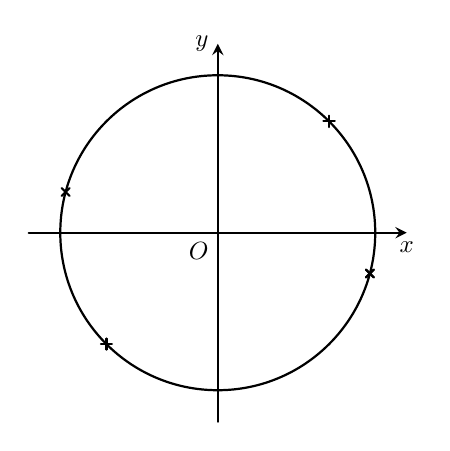
\begin{tikzpicture}[line join=round, line cap=round,>=stealth,thick]
\tikzset{every node/.style={scale=0.9}}
\draw[->] (-2.4,0)--(2.4,0) node[below] {$x$};
\draw[->] (0,-2.4)--(0,2.4) node[left] {$y$};
\draw (0,0) node [below left] {$O$};
\draw (0,0) circle (2);
\foreach \i in {0,...,2}
{
\draw plot[mark=+] coordinates {({45+\i*360/2}:2)};
}
\foreach \i in {0,...,2}
{
\draw plot[mark=x] coordinates {({-15+\i*360/2}:2)};
}
\end{tikzpicture}
\end{center}
Vậy có tất cả 4 vị trí biểu diễn các nghiệm các nghiệm của phương trình.}
\end{ex}

\begin{ex}%[1K1B4-3]%[Chuyên đề Toán 11 - 2023]%[Dương Phước Sang, dự án WTB - Toán 11 - new 2023]
Nghiệm của phương trình $\cot \left( x+\dfrac{\pi}{3} \right)=\sqrt{3}$ có dạng $x=-\dfrac{\pi}{m}+\dfrac{k\pi}{n}$, với $k \in \mathbb{Z}$ và $m$, $n \in \mathbb{N}^*$. Khi đó $m-n$ bằng
\choice
{$-5$}
{\True $5$}
{$3$}
{$-3$}
\loigiai{
Ta có $\cot \left( x+\dfrac{\pi}{3} \right)=\sqrt{3}$ $\Leftrightarrow \cot \left( x+\dfrac{\pi}{3} \right)=\cot \dfrac{\pi}{6}$ $\Leftrightarrow x+\dfrac{\pi}{3}=\dfrac{\pi}{6}+k\pi$ $\Leftrightarrow x=-\dfrac{\pi}{6}+k\pi$, $\left( k \in \mathbb{Z} \right)$.\\
Vậy $\heva{&m=6\\&n=1}$ $\Rightarrow m-n=5$.
}
\end{ex}

\begin{ex}%[1K1B4-3]%[Chuyên đề Toán 11 - 2023]%[Dương Phước Sang, dự án WTB - Toán 11 - new 2023]
Họ nghiệm của phương trình $\tan \left( x-\dfrac{\pi}{4} \right)-1=0$ là
\choice
{\True $x=\dfrac{\pi}{2}+k\pi$, $k \in \mathbb{Z}$}
{$x=k\pi$, $k \in \mathbb{Z}$}
{$x=\dfrac{\pi}{2}+k2\pi$, $k \in \mathbb{Z}$}
{$x=\dfrac{\pi}{4}+k\pi$, $k \in \mathbb{Z}$}
\loigiai{
Ta có $\tan \left( x-\dfrac{\pi}{4} \right)-1=0 \Leftrightarrow \tan \left( x-\dfrac{\pi}{4} \right)=1 \Leftrightarrow x-\dfrac{\pi}{4}=\dfrac{\pi}{4}+k\pi \Leftrightarrow x=\dfrac{\pi}{2}+k\pi$.\\
Vậy nghiệm của phương trình là $x=\dfrac{\pi}{2}+k\pi$, $k \in \mathbb{Z}$.
}
\end{ex}

\begin{ex}%[1K1B4-4]%[Chuyên đề Toán 11 - 2023]%[Dương Phước Sang, dự án WTB - Toán 11 - new 2023]
Phương trình $\tan\left(3x-15^{\circ}\right)=\sqrt{3}$ có các nghiệm là
\choice
{$x=60^{\circ}+k180^{\circ}$}
{$x=75^{\circ}+k180^{\circ}$}
{$x=75^{\circ}+k60^{\circ}$}
{\True $x=25^{\circ}+k60^{\circ}$}
\loigiai{
Ta có $\tan\left(3x-15^{\circ}\right)=\sqrt{3} \Leftrightarrow \tan\left(3x-15^{\circ}\right)=\tan 60^{\circ} \Leftrightarrow 3x-15^{\circ}=60^{\circ}+k180^{\circ}$ $ \Leftrightarrow x=25^{\circ}+k60^{\circ}$ $(k \in \mathbb{Z})$.
}
\end{ex}

\begin{ex}%[1K1B4-3]
Họ nghiệm của phương trình $\sin x=\sin\dfrac{\pi}{5}$ là
\choice
{$\left[\begin{aligned}
& x=\dfrac{\pi}{5}+k\pi\\
& x=\dfrac{4\pi}{5}+l\pi\\
\end{aligned}\right.,\,k,l\in\mathbb{Z}$}
{\True $\left[\begin{aligned}
& x=\dfrac{\pi}{5}+k2\pi\\
& x=\dfrac{4\pi}{5}+l2\pi\\
\end{aligned}\right.,\,k,l\in\mathbb{Z}$}
{$\left[\begin{aligned}
& x=\dfrac{\pi}{5}+k2\pi\\
& x=-\dfrac{\pi}{5}+l2\pi\\
\end{aligned}\right.,\,k,l\in\mathbb{Z}$}
{$\left[\begin{aligned}
& x=\dfrac{\pi}{5}+k\pi\\
& x=-\dfrac{\pi}{5}+l\pi\\
\end{aligned}\right.,\,k,l\in\mathbb{Z}$}
\loigiai{
Áp dụng công thức nghiệm của phương trình $\sin x=\sin\alpha\Leftrightarrow\left[\begin{aligned}
& x=\alpha+k2\pi\\
& x=\pi-\alpha+l2\pi\\
\end{aligned}\right.,\,k,\,l\in\mathbb{Z}$.\\
Ta có $\sin x=\sin\dfrac{\pi}{5}$$\Leftrightarrow\left[\begin{aligned}
& x=\dfrac{\pi}{5}+k2\pi\\
& x=\dfrac{4\pi}{5}+l2\pi\\
\end{aligned}\right.,\,k,l\in\mathbb{Z}$.}
\end{ex}

\begin{ex}%[Chuyên đề Toán 11 - 2023]%[Quan Ón, dự án WTB - Toán 11 - new 2023]%[1K1B4-5]
Phương trình $8 \cdot \cos 2x \cdot \sin 2x \cdot \cos 4x=-\sqrt{2}$ có nghiệm là
\choice
{\True $\hoac{&x=\dfrac{-\pi}{32}+k\dfrac{\pi}{4}\\&x=\dfrac{5\pi}{32}+k\dfrac{\pi}{4}}\left( k \in \mathbb{Z} \right)$}
{$\hoac{&x=\dfrac{\pi}{16}+k\dfrac{\pi}{8}\\&x=\dfrac{3\pi}{16}+k\dfrac{\pi}{8}}\left( k \in \mathbb{Z} \right)$}
{$\hoac{&x=\dfrac{\pi}{8}+k\dfrac{\pi}{8}\\&x=\dfrac{3\pi}{8}+k\dfrac{\pi}{8}}\left( k \in \mathbb{Z} \right)$}
{$\hoac{&x=\dfrac{\pi}{32}+k\dfrac{\pi}{4}\\&x=\dfrac{3\pi}{32}+k\dfrac{\pi}{4}}\left( k \in \mathbb{Z} \right)$}
\loigiai{
Ta có
\begin{eqnarray*}
8 \cdot \cos 2x \cdot \sin 2x \cdot \cos 4x=-\sqrt{2} \Leftrightarrow 4 \cdot \sin 4x \cdot \cos 4x=-\sqrt{2}
& \Leftrightarrow &2 \cdot \sin 8x=-\sqrt{2} \Leftrightarrow \sin 8x=-\dfrac{\sqrt{2}}{2}\\
&\Leftrightarrow& \sin 8x=\sin \left( -\dfrac{\pi}{4} \right)\\
&\Leftrightarrow& \hoac{&x=-\dfrac{\pi}{32}+k\dfrac{\pi}{4}\\&x=\dfrac{5\pi}{32}+k\dfrac{\pi}{4}}\left( k \in \mathbb{Z} \right).
\end{eqnarray*}
Vậy phương trình có nghiệm $\hoac{&x=\dfrac{-\pi}{32}+k\dfrac{\pi}{4}\\&x=\dfrac{5\pi}{32}+k\dfrac{\pi}{4}}\left( k \in \mathbb{Z} \right)$.
}
\end{ex}

\begin{ex}%[1K1B4-3]%[Chuyên đề Toán 11 - 2023]%[Dương Phước Sang, dự án WTB - Toán 11 - new 2023]
Phương trình lượng giác $\sqrt{3} \cdot \tan x+3=0$ có nghiệm là
\choice
{$x=\dfrac{\pi}{3}+k\pi$}
{$x=-\dfrac{\pi}{3}+k2\pi$}
{$x=\dfrac{\pi}{6}+k\pi$}
{\True $x=-\dfrac{\pi}{3}+k\pi$}
\loigiai{
Ta có $\sqrt{3} \cdot \tan x+3=0 \Leftrightarrow \tan x=-\sqrt{3} \Leftrightarrow x=-\dfrac{\pi}{3}+k\pi$ $(k \in \mathbb{Z})$.
}
\end{ex}

\begin{ex}%[1K1B4-3]
Nghiệm của phương trình $\cos x=\dfrac{1}{2}$ là
\choice
{$x=\pm \dfrac{\pi}{2}+k2\pi$}
{\True $x=\pm \dfrac{\pi}{3}+k2\pi$}
{$x=\pm \dfrac{\pi}{4}+k2\pi $}
{$x=\pm \dfrac{\pi}{6}+k2\pi $}
\loigiai{
Ta có $\cos x=\dfrac{1}{2}\Leftrightarrow \cos x=\cos \dfrac{\pi}{3}\Leftrightarrow x=\pm \dfrac{\pi}{3}+k2\pi \quad (k\in \mathbb{Z})$.}
\end{ex}

\begin{ex}%[Thành Đức Trung, Hàm số - Đợt 2 - Tư duy mở]%[1K1B4-9]
Giá trị lớn nhất của hàm số $y = \dfrac{\cos x + 2\sin x}{2\cos x+\sin x+3}$ bằng
\choice
{\True $\dfrac{1}{2}$}
{$\dfrac{5}{2}$}
{$4$}
{$\dfrac{3}{4}$}
\loigiai
{
Tập xác định $\mathscr{D}=\mathbb{R}$. \\
Ta có
\[\begin{aligned}
y = \dfrac{\cos x + 2\sin x}{2\cos x+\sin x+3}&\Leftrightarrow y\left(2\cos x + \sin x + 3\right) = \cos x + 2\sin x\\
&\Leftrightarrow (2y - 1)\cos x + (y - 2)\sin x = -3y.
\end{aligned}\]
Điều kiện để phương trình trên có nghiệm là
\[(2y - 1)^2 + (y - 2)^2 \ge (-3y)^2\Leftrightarrow 4y^2 + 8y - 5\le 0 \Leftrightarrow -\dfrac{5}{2}\le y\le \dfrac{1}{2}.\]
Vậy $\max\limits_{\mathbb{R}} y=\dfrac{1}{2}$.
}
\end{ex}

\begin{ex}%[1K1B4-3]
Phương trình $2\sin x-\sqrt{3}=0$ có tập nghiệm là
\choice
{$\left\{\pm\dfrac{\pi}{6}+k2\pi ,k\in\mathbb{Z}\right\}$}
{$\left\{\pm\dfrac{\pi}{3}+k2\pi ,k\in\mathbb{Z}\right\}$}
{$\left\{\dfrac{\pi}{6}+k2\pi ,\dfrac{5\pi}{6}+k2\pi ,k\in\mathbb{Z}\right\}$}
{\True $\left\{\dfrac{\pi}{3}+k2\pi ,\dfrac{2\pi}{3}+k2\pi ,k\in\mathbb{Z}\right\}$}
\loigiai{
$2\sin x-\sqrt{3}=0\Leftrightarrow\sin x=\dfrac{\sqrt{3}}{2}\Leftrightarrow\left[\begin{aligned}
& x=\dfrac{\pi}{3}+k2\pi\\
& x=\dfrac{2\pi}{3}+k2\pi\\
\end{aligned}\right.\left(k\in\mathbb{Z}\right).$\\
Vậy tập nghiệm của phương trình là  $S=\left\{\dfrac{\pi}{3}+k2\pi ,\dfrac{2\pi}{3}+k2\pi ,k\in\mathbb{Z}\right\}$}
\end{ex}

\begin{ex}%[1K1B4-5]
Tập nghiệm của phương trình $\cos 3x+\sin \dfrac{2\pi }{3}=0$ là
\choice
{\True $\left\{ \pm \dfrac{5\pi }{18}+\dfrac{k2\pi }{3}, k\in \mathbb{Z} \right\}$}
{$\left\{ \pm \dfrac{2\pi }{9}+\dfrac{k2\pi }{3}, k\in \mathbb{Z} \right\}$}
{$\left\{ \pm \dfrac{5\pi }{9}+\dfrac{k2\pi }{3}, k\in \mathbb{Z} \right\}$}
{$\left\{ \pm \dfrac{5\pi }{12}+\dfrac{k2\pi }{3}, k\in \mathbb{Z} \right\}$}
\loigiai{
Ta có
\allowdisplaybreaks
\begin{eqnarray*}
&&\cos 3x+\sin \dfrac{2\pi }{3}=0\\
&\Leftrightarrow& \cos 3x=-\sin \dfrac{2\pi }{3}\\
&\Leftrightarrow& \cos 3x=\cos \dfrac{5\pi }{6}
\Leftrightarrow 3x=\pm \dfrac{5\pi }{6}+k2\pi\Leftrightarrow x=\pm \dfrac{5\pi }{18}+\dfrac{k2\pi }{3} \quad (k\in \mathbb{Z}).
\end{eqnarray*}
}
\end{ex}


\begin{ex}%[1K1K4-3]
Tìm tổng các nghiệm của phương trình $\cos\left(5x-\dfrac{\pi}{6}\right)=\cos\left(2x-\dfrac{\pi}{3}\right)$ trên $\left[0\,;\pi\right]$.
\choice
{\True $\dfrac{47\pi}{18}$}
{$\dfrac{4\pi}{18}$}
{$\dfrac{45\pi}{18}$}
{$\dfrac{7\pi}{18}$}
\loigiai{
Ta có \\
$\cos\left(5x-\dfrac{\pi}{6}\right)=\cos\left(2x-\dfrac{\pi}{3}\right)$ $\Leftrightarrow\left[\begin{aligned}
& 5x-\dfrac{\pi}{6}=2x-\dfrac{\pi}{3}+k2\pi\\
& 5x-\dfrac{\pi}{6}=-2x+\dfrac{\pi}{3}+k2\pi\\
\end{aligned}\right.,k\in\mathbb{Z}$ $\Leftrightarrow\left[\begin{aligned}
& x=-\dfrac{\pi}{18}+\dfrac{k2\pi}{3}\\
& x=\dfrac{\pi}{14}+\dfrac{k2\pi}{7}\\
\end{aligned}\right.,k\in\mathbb{Z}$ .\\
Vì $ x\in\left[0\,;\pi\right]$ nên ta có  \\
+) Với $x=-\dfrac{\pi}{18}+\dfrac{k2\pi}{3}\Rightarrow 0\le-\dfrac{\pi}{18}+\dfrac{k2\pi}{3}\le\pi\Leftrightarrow\dfrac{1}{12}\le k\le\dfrac{19}{12}$ , do $ k\in\mathbb{Z}\Rightarrow k=1$ nên $x=\dfrac{11\pi}{18}$ .\\
+) Với $x=\dfrac{\pi}{14}+\dfrac{k2\pi}{7}\Rightarrow 0\le\dfrac{\pi}{14}+\dfrac{k2\pi}{7}\le\pi\Leftrightarrow\dfrac{-1}{4}\le k\le\dfrac{13}{4}$ , do $ k\in\mathbb{Z}\Rightarrow k\in\left\{ 0;1;2;3\right\}$ nên $x\in\left\{\dfrac{\pi}{14};\dfrac{5\pi}{14};\dfrac{9\pi}{14};\dfrac{13\pi}{14}\right\}$ .\\
Tổng tất cả các nghiệm là  $\dfrac{11\pi}{18}+\dfrac{\pi}{14}+\dfrac{5\pi}{14}+\dfrac{9\pi}{14}+\dfrac{13\pi}{14}=\dfrac{47\pi}{18}$ .}
\end{ex}

\begin{ex}%[1K1K4-2]

\immini
{
Cung lượng giác có điểm biểu diễn là $M_1,\,\,M_2$ như hình vẽ là nghiệm của phương trình lượng giác nào sau đây?
\choice
{\True $\sin\left(x-\dfrac{\pi}{3}\right)=0$}
{$\sin x=0$}
{$\cos\left(x-\dfrac{\pi}{3}\right)=0$}
{$\sin\left(x+\dfrac{\pi}{3}\right)=0$}
}
{
\begin{tikzpicture}
\path (0,0)coordinate[label=below left:$O$](O) (1,0)coordinate[label=below right:$A$](A) (-1,0)coordinate[label=below left:$A'$](A') (0,1)coordinate[label=above left:$B$](B) (0,-1)coordinate[label=below left:$B'$](B') ;
\draw[line width=0.4pt,black] (O) circle (1cm);
\draw[->] (0,-2)--(0,2)node[right]{$y$};
\draw[->] (-2,0)--(2,0)node[below]{$x$};
\coordinate[label=right:$M_1$] (M1) at ($(O)+(60:1)$);
\coordinate[label=left:$M_2$] (M2) at ($(O)+(-120:1)$);
\coordinate  (O1) at ($(O)+(0:0.2)$);
%\coordinate  (O2) at ($(O)+(60:0.2)$);
\draw[line width=0.4pt,black,->] (O1) arc (0:60:0.2cm)node[right]{$\frac{\pi}{3}$};

\draw[dashed] (M1)--(M2);
\foreach \diem in {A,B,A',B',O,M1,M2} \fill[black](\diem)circle(1.5pt);

\end{tikzpicture}
}
\loigiai{
Cung lượng giác có điểm biểu diễn là $M_1,\,\,M_2$ có số đo là  $\dfrac{\pi}{3}+k\pi\,\,\left(k\in\mathbb{Z}\right)$.\\
Và phương trình $\sin\left(x-\dfrac{\pi}{3}\right)=0\Leftrightarrow x-\dfrac{\pi}{3}=k\pi\Leftrightarrow x=\dfrac{\pi}{3}+k\pi\,\,\left(k\in\mathbb{Z}\right)$.}
\end{ex}

\begin{ex}%[1K1K4-3]
Phương trình $\sin \left( 3x+\dfrac{\pi}{3} \right)=-\dfrac{\sqrt{3}}{2}$ có bao nhiêu nghiệm thuộc khoảng $\left( 0;\dfrac{\pi}{2} \right)$?
\choice
{$3$}
{$4$}
{$1$}
{\True $2$}
\loigiai{
\allowdisplaybreaks
\begin{eqnarray*}
&&\sin \left( 3x+\dfrac{\pi}{3} \right)=-\dfrac{\sqrt{3}}{2}\\
&\Leftrightarrow& \sin \left( 3x+\dfrac{\pi}{3} \right)=\sin \left( -\dfrac{\pi}{3} \right)\Leftrightarrow \hoac{&3x+\dfrac{\pi}{3}=-\dfrac{\pi}{3}+k2\pi\\&3x+\dfrac{\pi}{3}=\pi +\dfrac{\pi}{3}+k2\pi} \Leftrightarrow \hoac{&x=-\dfrac{2\pi }{9}+\dfrac{k2\pi }{3}\\&x=\dfrac{\pi}{3}+\dfrac{k2\pi }{3}} \quad (k\in \mathbb{Z}).
\end{eqnarray*}
\begin{itemize}
\item $x=-\dfrac{2\pi }{9}+\dfrac{k2\pi }{3}\in \left( 0;\dfrac{\pi}{2} \right)\Leftrightarrow 0<-\dfrac{2\pi }{9}+\dfrac{k2\pi }{3}<\dfrac{\pi}{2}\Leftrightarrow \dfrac{1}{3}<k<\dfrac{13}{12}$.\\
Do $k\in \mathbb{Z}\Rightarrow k=1$. Suy ra trường hợp này có nghiệm $x=\dfrac{4\pi }{9}$ thỏa mãn.
\item Với $x=\dfrac{\pi}{3}+\dfrac{k2\pi }{3}\in \left( 0;\dfrac{\pi}{2} \right)\Leftrightarrow 0<\dfrac{\pi}{3}+\dfrac{k2\pi }{3}<\dfrac{\pi}{2}\Leftrightarrow -\dfrac{1}{2}<k<\dfrac{1}{4}$. \\
Do $k\in \mathbb{Z}\Rightarrow k=0$. Suy ra trường hợp này có nghiệm $x=\dfrac{\pi}{3}$ thỏa mãn.
\end{itemize}
Vậy phương trình đã cho có  đúng $2$ nghiệm thuộc khoảng $\left( 0;\dfrac{\pi}{2} \right)$.}
\end{ex}

\begin{ex}%[1K1K4-3]
Tính tổng $S$ của các nghiệm của phương trình $\sin x=\dfrac{1}{2}$ trên đoạn $\left[ -\dfrac{\pi}{2};\dfrac{\pi}{2} \right]$.
\choice
{$S=\dfrac{5\pi}{6}$}
{$S=\dfrac{\pi}{3}$}
{$S=\dfrac{\pi}{2}$}
{\True $S=\dfrac{\pi}{6}$}
\loigiai{
Ta có $\sin x=\dfrac{1}{2}\Leftrightarrow \hoac{&x=\dfrac{\pi}{6}+2k\pi\\&x=\dfrac{5\pi }{6}+2k\pi} \quad (k\in \mathbb{Z}).$\\
Vì $x\in \left[ -\dfrac{\pi}{2};\dfrac{\pi}{2} \right]$ nên $x=\dfrac{\pi}{6}\Rightarrow S=\dfrac{\pi}{6}$.}
\end{ex}

\begin{ex}%[1K1K4-3]
Phương trình $ 2\sin x+\sqrt{3}=0$ có tổng nghiệm dương nhỏ nhất và nghiệm âm lớn nhất bằng
\choice
{$\dfrac{4\pi}{3}$}
{$ 2\pi $}
{$\dfrac{\pi}{3}$}
{\True $\pi $}
\loigiai{
* Ta có  $ 2\sin x+\sqrt{3}=0\Leftrightarrow\sin x=-\dfrac{\sqrt{3}}{2}=\sin\left(-\dfrac{\pi}{3}\right)\Leftrightarrow\left[\begin{array}{*{35}{l}}
x=-\dfrac{\pi}{3}+k2\pi\\
x=\dfrac{4\pi}{3}+k2\pi\\
\end{array}\right.\,\,\,\,\,,k\in\mathbb{Z}$.\\
* Xét $ x=-\dfrac{\pi}{3}+k2\pi $, $ k\in\mathbb{Z}$ ta được nghiệm dương nhỏ nhất là $x_1=\dfrac{5\pi}{3}$ và nghiệm âm lớn nhất là $x_2=-\dfrac{\pi}{3}$.\\
* Xét $ x=\dfrac{4\pi}{3}+k2\pi $, $ k\in\mathbb{Z}$ ta được nghiệm dương nhỏ nhất là $x_3=\dfrac{4\pi}{3}$ và nghiệm âm lớn nhất là $x_4=-\dfrac{2\pi}{3}$.\\
* So sánh $x_1$ và $x_3$ ta suy ra nghiệm dương nhỏ nhất của phương trình đã cho là $x_3=\dfrac{4\pi}{3}$.\\
So sánh $x_2$ và $x_4$ ta suy ra nghiệm âm lớn nhất của phương trình đã cho là $x_2=-\dfrac{\pi}{3}$.\\
* Ta có $x_2+x_3=-\dfrac{\pi}{3}+\dfrac{4\pi}{3}=\pi $.}
\end{ex}

\begin{ex}%[1K1K4-3]
Tìm số nghiệm của phương trình $\sin \left( \cos 2x \right)=0$ trên $\left[0; 2\pi\right].$
\choice
{$2$}
{$1$}
{\True $4$}
{$3$}
\loigiai{
Ta có $\sin \left(\cos2x \right)=0\Leftrightarrow \cos2x=k\pi \quad (k\in \mathbb{Z}).$\\
Vì $\cos2x\in \left[-1;1 \right]\Rightarrow k=0$.\\
Lúc đó phương trình trở thành $\cos2x=0\Leftrightarrow 2x=\dfrac{\pi}{2}+k\pi \Leftrightarrow x=\dfrac{\pi}{4}+\dfrac{h\pi}{2} \quad (h\in \mathbb{Z}).$\\
$x\in \left[ 0;2\pi \right]\Rightarrow h \in \left\{ 0;1;2;3 \right\}.$
Vậy phương trình có $4$ nghiệm trên $\left[0; 2\pi \right].$}
\end{ex}

\begin{ex}%[Chuyên đề Toán 11 - 2023]%[Quan Ón, dự án WTB - Toán 11 - new 2023]%[1K1K4-5]
Giải phương trình $\cot x+\sin x\left( 1+\tan x \cdot \tan \dfrac{x}{2} \right)=4$, ta được họ nghiệm là
\choice
{\True $\hoac{&x = \dfrac{\pi}{12} + k\pi \\&x = \dfrac{5\pi}{12} + k\pi}$, $\left( k \in \mathbb{Z} \right)$}
{$\hoac{&x = \dfrac{\pi}{2} + k2\pi \\&x = \dfrac{\pi}{6} + k2\pi}$, $\left( k \in \mathbb{Z} \right)$}
{$\hoac{&x = \dfrac{\pi}{3} + k\pi \\&x = \dfrac{5\pi}{6} + k\pi}$, $\left( k \in \mathbb{Z} \right)$}
{$\hoac{&x=k\pi \\&x=\pm \dfrac{\pi}{3}+k2\pi}$, $\left( k \in \mathbb{Z} \right)$}
\loigiai{
ĐK: $\heva{&\sin x \ne 0\\&\cos \dfrac{x}{2} \ne 0\\&\cos x \ne 0}$ $\Leftrightarrow \heva{&\sin 2x \ne 0\\&\cos \dfrac{x}{2} \ne 0} \Leftrightarrow x \ne \dfrac{k\pi}{2}, \left( k \in \mathbb{Z} \right)$.\\
$\cot x+\sin x\left( 1+\tan x \cdot \tan \dfrac{x}{2} \right)=4$\\
$\Leftrightarrow \dfrac{\cos x}{\sin x}+\sin x\left( 1+\dfrac{\sin x}{\cos x} \cdot \dfrac{\sin \dfrac{x}{2}}{\cos \dfrac{x}{2}} \right)=4$ $\Leftrightarrow \dfrac{\cos x}{\sin x}+\sin x\left( \dfrac{\cos x \cdot \cos \dfrac{x}{2}+\sin x \cdot \sin \dfrac{x}{2}}{\cos x \cdot \cos \dfrac{x}{2}} \right)=4$\\
$\Leftrightarrow \dfrac{\cos x}{\sin x}+\sin x\left( \dfrac{\cos \left( x-\dfrac{x}{2} \right)}{\cos x \cdot \cos \dfrac{x}{2}} \right)=4$ $\Leftrightarrow \dfrac{\cos x}{\sin x}+\dfrac{\sin x}{\cos x}=4$ $\Leftrightarrow 4\sin x\cos x=1$\\
$\Leftrightarrow \sin 2x=\dfrac{1}{2}$ $\Leftrightarrow \hoac{&x=\dfrac{\pi}{12}+k\pi \\&x=\dfrac{5\pi}{12}+k\pi}, \left( k \in \mathbb{Z} \right)$ thỏa mãn điều kiện.\\
Vậy nghiệm của phương trình đã cho là $x=\dfrac{\pi}{12}+k\pi$; $x=\dfrac{5\pi}{12}+k\pi$ $\left( k \in \mathbb{Z} \right)$.
}
\end{ex}

\begin{ex}%[1K1K4-3]%[Chuyên đề Toán 11 - 2023]%[Dương Phước Sang, dự án WTB - Toán 11 - new 2023]
Số nghiệm của phương trình $\cot 20x=1$ trên đoạn $\left[ -50\pi;0 \right]$ là
\choice
{$980$}
{$1001$}
{\True $1000$}
{$981$}
\loigiai{
Ta có $\cot 20x=1 \Leftrightarrow 20x=\dfrac{\pi}{4}+k\pi \Leftrightarrow x=\dfrac{\pi}{80}+k\dfrac{\pi}{20}$, $k \in \mathbb{Z}$.\\
Với $x=\dfrac{\pi}{80}+k\dfrac{\pi}{20}$ và $-50\pi \leq x \leq 0$, ta có $-50\pi \leq \dfrac{\pi}{80}+k\dfrac{\pi}{20} \leq 0 \Leftrightarrow -50\pi -\dfrac{\pi}{80} \leq k\dfrac{\pi}{20} \leq -\dfrac{\pi}{80}$\\
\[\Leftrightarrow -1000-\dfrac{1}{4} \leq k \leq -\dfrac{1}{4},\;k \in \mathbb{Z}. \text{ Do đó } k \in \big\{-1000;-999;\ldots;-1\big\}.\]
Vậy phương trình đã cho có $1000$ nghiệm trên $\left[ -50\pi;0 \right]$.
}
\end{ex}

\begin{ex}%[1K1K4-3]
Có bao nhiêu nghiệm phương trình $\sin 2x=-\dfrac{\sqrt{2}}{2}$ trong khoảng $\left( 0;\pi \right)$?
\choice
{$4$}
{$3$}
{\True $2$}
{$1$}
\loigiai{
$\sin 2x=-\dfrac{\sqrt{2}}{2}\Leftrightarrow
\hoac{&2x=\dfrac{-\pi }{4}+k2\pi\\&2x=\dfrac{5\pi }{4}+k2\pi}\Leftrightarrow \hoac{&x=\dfrac{-\pi }{8}+k\pi\\&x=\dfrac{5\pi }{8}+k\pi} \quad (k\in \mathbb{Z}).$\\
\textbf{TH1:} $x=-\dfrac{\pi}{8}+k\pi\in (0;\pi) \Leftrightarrow 0<-\dfrac{\pi }{8}+k\pi <\pi \Leftrightarrow \dfrac{1}{8}<k<\dfrac{9}{8}$. Vì $k\in \mathbb{Z}$ nên $k=1$.\\
\textbf{TH2:} $x=\dfrac{5\pi}{8}+k\pi\in (0;\pi) \Leftrightarrow 0<\dfrac{5\pi }{8}+k\pi <\pi \Leftrightarrow \dfrac{-5}{8}<k<\dfrac{3}{8}$. Vì $k\in \mathbb{Z}$ nên $k=0$.\\
Vậy phương trình đã cho có 2 nghiệm trong khoảng $(0;\pi)$.
}
\end{ex}

\begin{ex}%[1K1K4-3]%[Chuyên đề Toán 11 - 2023]%[Dương Phước Sang, dự án WTB - Toán 11 - new 2023]
Trong các phương trình sau đây, phương trình nào có nghiệm dương nhỏ nhất nhỏ hơn nghiệm dương của các phương trình còn lại?
\choice
{\True $\tan 2x=1$}
{$\tan\left(x-\dfrac{\pi}{4}\right)=\sqrt{3}$}
{$\cot x=0$}
{$\cot x=-\sqrt{3}$}
\loigiai{
\begin{itemize}
\item $\tan 2x=1 \Leftrightarrow \tan 2x=\tan\dfrac{\pi}{4} \Leftrightarrow 2x=\dfrac{\pi}{4}+k\pi \Leftrightarrow x=\dfrac{\pi}{8}+k\dfrac{\pi}{2}$ $(k \in \mathbb{Z})$.\\
Nghiệm dương bé nhất của phương trình này là $x=\dfrac{\pi}{8}$.
\item $\tan\left(x-\dfrac{\pi}{4}\right)=\sqrt{3} \Leftrightarrow x-\dfrac{\pi}{4}=\dfrac{\pi}{3}+k\pi \Leftrightarrow x=\dfrac{7\pi}{12}+k\pi$ $(k \in \mathbb{Z})$.\\
Nghiệm dương bé nhất của phương trình này là $x=\dfrac{7\pi}{12}$.
\item $\cot x=0 \Leftrightarrow \cos x=0 \Leftrightarrow x=\dfrac{\pi}{2}+k\pi$ $(k \in \mathbb{Z})$.\\
Nghiệm dương bé nhất của phương trình này là $x=\dfrac{\pi}{2}$.
\item $\cot x=-\sqrt{3} \Leftrightarrow \cot x=\cot\left(-\dfrac{\pi}{6}\right) \Leftrightarrow x=-\dfrac{\pi}{6}+k\pi$ $(k \in \mathbb{Z})$.\\

Nghiệm dương bé nhất của phương trình này là $x=\dfrac{5\pi}{6}$.
\end{itemize}
Vậy giá trị nhỏ nhất là $x=\dfrac{\pi}{8}$ nên ta chọn $\tan 2x=1$.
}
\end{ex}

\begin{ex}%[1K1K4-3]
Cho phương trình $2\sin x-\sqrt{3}=0$. Tổng các nghiệm thuộc $\left[ 0;\pi \right]$ của phương trình là
\choice
{$\dfrac{4\pi }{3}$}
{\True $\pi$}
{$\dfrac{\pi}{3}$}
{$\dfrac{2\pi }{3}$}
\loigiai{
Ta có $2\sin x-\sqrt{3}=0\Leftrightarrow \sin x=\dfrac{\sqrt{3}}{2}=\sin \dfrac{\pi}{3}\Leftrightarrow\hoac{& x=\dfrac{\pi}{3}+k2\pi\\& x=\dfrac{2\pi }{3}+k2\pi} \quad (k\in \mathbb{Z})$.\\
Các nghiệm của phương trình trong đoạn $\left[0;\pi \right]$ là $\dfrac{\pi}{3}$; $\dfrac{2\pi }{3}$ nên có tổng là $\dfrac{\pi}{3}+\dfrac{2\pi }{3}=\pi $.}
\end{ex}

\begin{ex}%[1K1K4-3]
Cho phương trình $\sin \left( 2x-\dfrac{\pi}{4} \right)=\sin \left( x+\dfrac{3\pi }{4} \right)$. Tính tổng các nghiệm thuộc khoảng$\left( 0;\pi \right)$ của phương trình trên.
\choice
{$\dfrac{7\pi }{2}$}
{\True $\pi $}
{$\dfrac{3\pi }{2}$}
{$\dfrac{\pi}{4}$}
\loigiai{
Ta có $\sin \left( 2x-\dfrac{\pi}{4} \right)=\sin \left( x+\dfrac{3\pi }{4} \right)\Leftrightarrow \hoac{&2x-\dfrac{\pi}{4}=x+\dfrac{3\pi }{4}+k2\pi \\&2x-\dfrac{\pi}{4}=\pi -x-\dfrac{3\pi }{4}+k2\pi} \Leftrightarrow \hoac{&x=\pi +k2\pi\\&x=\dfrac{\pi}{6}+\dfrac{k2\pi }{3}} \quad (k\in \mathbb{Z}).$
\begin{itemize}
\item Xét $x=\pi +k2\pi$.\\
$x\in (0;\pi) \Leftrightarrow 0<\pi +k2\pi <\pi \Leftrightarrow -\dfrac{1}{2}<k<0$. Vì $k\in \mathbb{Z}$ nên không có giá trị $k$.
\item  Xét $x=\dfrac{\pi}{6}+\dfrac{k2\pi }{3}$.\\
$x\in (0;\pi) \Leftrightarrow 0<\dfrac{\pi}{6}+\dfrac{k2\pi }{3}<\pi \Leftrightarrow -\dfrac{1}{4}<k<\dfrac{5}{4}$. Vì $k\in \mathbb{Z}$ nên có hai giá trị $k$ là: $k=0;k=1$. \\
Khi đó ta có các nghiệm tương ứng là $x=\dfrac{\pi}{6}$ và $x=\dfrac{5\pi}{6}$.
\end{itemize}
Vậy tổng các nghiệm của phương trình đã cho trong khoảng $\left( 0;\pi \right)$ là: $\dfrac{\pi}{6}+\dfrac{5\pi }{6}=\pi $.}
\end{ex}

\begin{ex}%[1K1K4-3]
Số nghiệm thực của phương trình $ 2\sin x-1=0$ trên đoạn $\left[-\dfrac{3\pi}{2}\,;\,\,10\pi\right]$ là
\choice
{\True $11$}
{$9$}
{$20$}
{$21$}
\loigiai{
Phương trình tương đương: $\sin x=\dfrac{1}{2}$ $\Leftrightarrow\left[\begin{aligned}
& x=\dfrac{\pi}{6}+k2\pi\\
& x=\dfrac{5\pi}{6}+k2\pi\\
\end{aligned}\right.$,\\
+Với $ x=\dfrac{\pi}{6}+k2\pi $, $k\in\mathbb{Z}$ ta có $-\dfrac{3\pi}{2}\le\dfrac{\pi}{6}+k2\pi\le 10\pi $, $k\in\mathbb{Z}$ $\Leftrightarrow-\dfrac{5}{6}\le k\le\dfrac{59}{12}$, $k\in\mathbb{Z}$\\
$\Rightarrow 0\le k\le 4$, $k\in\mathbb{Z}$ . Do đó phương trình có $ 5$ nghiệm.\\
+Với $ x=\dfrac{5\pi}{6}+k2\pi $, $k\in\mathbb{Z}$ ta có $-\dfrac{3\pi}{2}\le\dfrac{5\pi}{6}+k2\pi\le 10\pi $, $k\in\mathbb{Z}$ $\Leftrightarrow-\dfrac{7}{6}\le k\le\dfrac{55}{12}$, $k\in\mathbb{Z}$\\
$\Rightarrow-1\le k\le 4$, $k\in\mathbb{Z}$ . Do đó, phương trình có $ 6$ nghiệm.\\
+Rõ ràng các nghiệm này khác nhau từng đôi một, vì nếu\\
$\dfrac{\pi}{6}+k2\pi=\dfrac{5\pi}{6}+k'2\pi\Leftrightarrow k-k'=\dfrac{1}{3}$ .\\
Vậy phương trình có $ 11$ nghiệm trên đoạn $\left[-\dfrac{3\pi}{2}\,;\,\,10\pi\right]$.}
\end{ex}

\begin{ex}%[1K1K4-4]
Tổng các nghiệm của phương trình $ 2\sin\left(x+40^\circ\right)=\sqrt{3}$ trên khoảng $\left(-180^\circ\,;\,180^\circ\right)$ là
\choice
{$ 20^\circ $}
{\True $ 100^\circ $}
{$ 80^\circ $}
{$ 120^\circ $}
\loigiai{
Ta có  $2\sin\left(x+40^\circ\right)=\sqrt{3}$ $\Leftrightarrow\sin\left(x+40^\circ\right)=\dfrac{\sqrt{3}}{2}$\\
$\Leftrightarrow\left[\begin{aligned}
& x+40^\circ=60^\circ+k360^\circ\\
& x+40^\circ=120^\circ+k360^\circ\\
\end{aligned}\right.\left(k\in\mathbb{Z}\right)$ $\Leftrightarrow\left[\begin{aligned}
& x=20^\circ+k360^\circ\\
& x=80^\circ+k360^\circ\\
\end{aligned}\right.\left(k\in\mathbb{Z}\right)$\\
Theo đề bài:\\
$-180^\circ <20^\circ+k360^\circ <180^\circ\Leftrightarrow-\dfrac{5}{9}<k<\dfrac{4}{9}\Rightarrow k=0\Rightarrow x=20^\circ $ .\\
$-180^\circ <80^\circ+k360^\circ <180^\circ\Leftrightarrow-\dfrac{13}{18}<k<\dfrac{5}{18}\Rightarrow k=0\Rightarrow x=80^\circ $ .\\
Vậy tổng các nghiệm của phương trình là $ 20^\circ+80^\circ=100^\circ $.}
\end{ex}

\begin{ex}%[1K1K4-3]%[Chuyên đề Toán 11 - 2023]%[Dương Phước Sang, dự án WTB - Toán 11 - new 2023]
Phương trình $\cot 3x=\cot x$ có các nghiệm là
\choice
{$x=\dfrac{\pi}{2}+k2\pi$, $k \in \mathbb{Z}$}
{$x=k\pi$, $k \in \mathbb{Z}$}
{$x=\dfrac{k\pi}{3}$, $k \in \mathbb{Z}$}
{\True $x=\dfrac{\pi}{2}+k\pi$, $k \in \mathbb{Z}$}
\loigiai{
Điều kiện: $\heva{&\sin 3x \ne 0\\&\sin x \ne 0} \Leftrightarrow \heva{&x \ne k\dfrac{\pi}{3}\\&x \ne l\pi}$ $(k,l \in \mathbb{Z})$. $(*)$\\
Khi đó phương trình $\cot 3x=\cot x \Leftrightarrow 3x=x+k\pi \Leftrightarrow x=\dfrac{k\pi}{2}$ $(k \in \mathbb{Z})$.\\
Kết hợp điều kiện ta được các nghiệm của phương trình $x=\dfrac{\pi}{2}+k\pi$ $(k \in \mathbb{Z})$.\\
}
\end{ex}

\begin{ex}%[Thành Đức Trung, Hàm số - Đợt 2 - Tư duy mở]%[1K1K4-9]
Cho hai số thực $x$, $y$ thỏa mãn $x^{2}+y^{2}=1$. Gọi giá trị lớn nhất và giá trị nhỏ nhất của biểu thức $P=\dfrac{x^{2}+x y+1}{y^{2}-x y+2}$ lần lượt là $M$ và $m$. Giá trị của biểu thức $T=M+m$ bằng
\choice
{$12$}
{$\dfrac{5}{2}$}
{\True $\dfrac{34}{23}$}
{$\dfrac{27}{16}$}
\loigiai
{
Đặt $\heva{ & x=\cos t \\ & y=\sin t}$ với $t\in[0;2\pi]$, khi đó
\[ P=\dfrac{\cos ^{2} t+\cos t \cdot \sin t+1}{\sin ^{2} t-\cos t \cdot \sin t+2}=\dfrac{\dfrac{1+\cos 2 t}{2}+\dfrac{1}{2} \sin 2 t+1}{\dfrac{1-\cos 2 t}{2}-\frac{1}{2} \sin 2 t+2}=\dfrac{\cos 2 t+\sin 2 t+3}{-\cos 2 t-\sin 2 t+5}.\]
Suy ra $(P+1) \cos 2 t+(P+1) \sin 2 t=5 P-3$. \\
Điều kiện để có nghiệm $t$ là \[(P+1)^{2}+(P+1)^{2} \geq(5 P-3)^{2} \Leftrightarrow 23 P^{2}-34 P+7 \leq 0 \Leftrightarrow \frac{17-8 \sqrt{2}}{23} \leq P \leq \frac{17+8 \sqrt{2}}{23}.\]
Vậy $M=\max P=\dfrac{17+8 \sqrt{2}}{23} $; $m=\min P=\dfrac{17-8 \sqrt{2}}{23}$ và $T=M+m=\dfrac{34}{23}$.
}
\end{ex}

\begin{ex}%[1K1K4-3]
Số nghiệm của phương trình $\sin \left( x+\dfrac{\pi}{4} \right)=1$ với $\pi \le x\le 5\pi $ là
\choice
{$1$}
{$0$}
{$2$}
{\True $3$}
\loigiai{
Ta có $\sin \left( x+\dfrac{\pi}{4} \right)=1\Leftrightarrow x+\dfrac{\pi}{4}=\dfrac{\pi}{2}+k2\pi \Leftrightarrow x=\dfrac{\pi}{4}+k2\pi \quad (k\in \mathbb{Z}).$\\
Nên $\pi \le x\le 5\pi \Leftrightarrow \pi \le \dfrac{\pi}{4}+k2\pi \le 5\pi \Leftrightarrow \dfrac{3}{8}\le k\le \dfrac{19}{8}$
Vì $k\in \mathbb{Z}$ nên $k\in \left\{ 1;\,2;\,3 \right\}$.\\
Vậy phương trình đã cho có 3 nghiệm thuộc đoạn $[\pi;5\pi]$.
}
\end{ex}

\begin{ex}%[Chuyên đề Toán 11 - 2023]%[Quan Ón, dự án WTB - Toán 11 - new 2023]%[1K1K4-5]
Giải phương trình sau $4\sin x=\dfrac{\sqrt{3}}{\cos x}-\dfrac{2\sqrt{3}\sin 3x}{\sin 2x}$, ta được họ nghiệm là
\choice
{$x = \dfrac{\pi}{3}+k2\pi$, $\left( k \in \mathbb{Z} \right)$}
{\True $x = \dfrac{\pi}{3}+k\dfrac{\pi}{2}$, $\left( k \in \mathbb{Z} \right)$}
{$x = \dfrac{\pi}{4}+k\dfrac{\pi}{2}$, $\left( k \in \mathbb{Z} \right)$}
{$x = \pm\dfrac{\pi}{3}+k\pi$, $\left( k \in \mathbb{Z} \right)$}
\loigiai{
Điều kiện: $\sin 2x \ne 0 \Leftrightarrow x \ne k\dfrac{\pi}{2}\left( k \in \mathbb{Z} \right)$.\\
Ta có:
\begin{eqnarray*}
& & 4\sin x = \dfrac{\sqrt{3}}{\cos x}-\dfrac{2\sqrt{3}\sin 3x}{\sin 2x}\\
&\Leftrightarrow& 4\sin^2x\cos x=\sqrt{3}\sin x-\sqrt{3}\sin 3x\\
&\Leftrightarrow& 2\left( 1-\cos 2x \right)\cos x=\sqrt{3}\sin x-\sqrt{3}\sin 3x\\
&\Leftrightarrow& 2\cos x-2\cos 2x\cos x=\sqrt{3}\sin x-\sqrt{3}\sin 3x\\
&\Leftrightarrow& 2\cos x-\left( \cos 3x+\cos x \right)=\sqrt{3}\sin x-\sqrt{3}\sin 3x\\
&\Leftrightarrow& \sqrt{3}\sin 3x-\cos 3x=\sqrt{3}\sin x-\cos x\\
&\Leftrightarrow& \sin \left( 3x-\dfrac{\pi}{6} \right)=\sin \left( x-\dfrac{\pi}{6} \right)\\
&\Leftrightarrow& \hoac{&x=k\pi \\&x=\dfrac{\pi}{3}+k\dfrac{\pi}{2}}\,\, \left( k \in \mathbb{Z} \right).
\end{eqnarray*}
So với điều kiện, suy ra phương trình có 1 họ nghiệm là $x=\dfrac{\pi}{3}+k\dfrac{\pi}{2}\left( k \in \mathbb{Z} \right)$.
}
\end{ex}

\begin{ex}%[1K1K4-3]
Phương trình $\sin \left( 2x-\dfrac{\pi}{4} \right)=\sin \left( x+\dfrac{3\pi }{4} \right)$ có tổng các nghiệm thuộc khoảng $\left( 0;\pi \right)$ bằng
\choice
{$\dfrac{7\pi }{2}$}
{\True $\pi$}
{$\dfrac{3\pi }{2}$}
{$\dfrac{\pi}{4}$}
\loigiai{
\allowdisplaybreaks
\begin{eqnarray*}
\sin \left( 2x-\dfrac{\pi}{4} \right)=\sin \left( x+\dfrac{3\pi }{4} \right)\Leftrightarrow \hoac{&2x-\dfrac{\pi}{4}=x+\dfrac{3\pi }{4}+k2\pi\\&2x-\dfrac{\pi}{4}=\dfrac{\pi}{4}-x+k2\pi}\Leftrightarrow \hoac{&x=\pi +k2\pi\\&x=\dfrac{\pi}{6}+\dfrac{k2\pi }{3}}\quad (k\in \mathbb{Z}).
\end{eqnarray*}
Họ nghiệm $x=\pi +k2\pi $ không có nghiệm nào thuộc khoảng $\left( 0;\,\,\pi \right)$.\\
Xét họ nghiệm $x=\dfrac{\pi}{6}+\dfrac{k2\pi }{3}$. Ta có $x\in \left( 0; \pi \right)\Leftrightarrow 0<\dfrac{\pi}{6}+\dfrac{k2\pi }{3}<\pi \Leftrightarrow k\in \left\{ 0; 1\right\}$.\\
Lúc đó ta có hai nghiệm tương ứng $x=\dfrac{\pi}{6}$ và $x=\dfrac{5\pi }{6}$. \\
Suy ra tổng các nghiệm thuộc khoảng $\left( 0; \pi \right)$ của phương trình này bằng $\pi$.}
\end{ex}

\begin{ex}%[1K1K4-3]%[Chuyên đề Toán 11 - 2023]%[Dương Phước Sang, dự án WTB - Toán 11 - new 2023]
Tính tổng các nghiệm trong đoạn $[0;30]$ của phương trình $\tan x=\tan 3x$.
\choice
{$55\pi $}
{$\dfrac{171\pi}{2}$}
{\True $45\pi $}
{$\dfrac{190\pi}{2}$}
\loigiai{
Điều kiện để phương trình có nghĩa $\heva{&\cos x \ne 0\\&\cos 3x \ne 0} \Leftrightarrow \heva{&x \ne \dfrac{\pi}{2}+k\pi \\&x \ne \dfrac{\pi}{6}+\dfrac{l\pi}{3}}$ $(k,l \in \mathbb{Z})$. $(*)$\\
Khi đó, phương trình $3x=x+k\pi \Leftrightarrow x=\dfrac{k\pi}{2}$.\\
So sánh với điều kiện $(*)$ ta chỉ nhận
$x=k\pi$ $(k \in \mathbb{Z})$.\\
Và do $x \in [0;30]$ nên $x \in \left\{ 0;\pi;2\pi;\ldots ;9\pi \right\}$.\\
Vậy, tổng các nghiệm trong đoạn $[0;30]$ của phương trình là $45\pi $.
}
\end{ex}

\begin{ex}%[1K1K4-4]%[Chuyên đề Toán 11 - 2023]%[Dương Phước Sang, dự án WTB - Toán 11 - new 2023]
Tổng các nghiệm phương trình $\tan \left(2x-15^{\circ}\right)=1$ trên khoảng $\left(-90^{\circ};90^{\circ}\right)$ bằng
\choice
{$30^{\circ}$}
{$-60^{\circ}$}
{$0^{\circ}$}
{\True $-30^{\circ}$}
\loigiai{
Ta có $\tan \left(2x-15^{\circ}\right)=1 \Leftrightarrow 2x-15^{\circ}=45^{\circ}+k180^{\circ} \Leftrightarrow x=30^{\circ}+k90^{\circ}$,
với $k \in \mathbb{Z}$.\\
Xét $-90^{\circ}<30^{\circ}+k90^{\circ}<90^{\circ} \Leftrightarrow -\dfrac{4}{3}<k<\dfrac{2}{3} \Rightarrow \hoac{&k=-1\\&k=0} \Rightarrow \hoac{&x_1=-60^{\circ}\\&x_2=30^{\circ}.}$\\
Vậy $x_1+x_2=-30^{\circ}$.
}
\end{ex}

\begin{ex}%[Chuyên đề Toán 11 - 2023]%[Quan Ón, dự án WTB - Toán 11 - new 2023]%[1K1K4-5]
Số nghiệm phương trình $\dfrac{\sin 3x}{\cos x+1}=0$ thuộc đoạn $\left[ 2\pi;4\pi \right]$ là
\choice
{$7$}
{\True $6$}
{$4$}
{$5$}
\loigiai{
Điều kiện: $\cos x+1 \ne 0 \Leftrightarrow x \ne \pi +k2\pi$.\\
Ta có $\dfrac{\sin 3x}{\cos x+1}=0 \Rightarrow \sin 3x=0 \Leftrightarrow x=\dfrac{k\pi}{3}$, $\left( k \in \mathbb{Z} \right)$.\\
So với điều kiện, nghiệm của phương trình là $x=\dfrac{k\pi}{3}$ với $k \in \mathbb{Z},k \ne 3(2l+1)$.\\
Vì $2\pi \leq x \leq 4\pi \Leftrightarrow 2\pi \leq \dfrac{k\pi}{3} \leq 4\pi \Leftrightarrow 6 \leq k \leq 12$ nên ta chọn $k \in \big\{6,7,8,10,11,12\big\}$.
}
\end{ex}

\begin{ex}%[1K1K4-3]%[Chuyên đề Toán 11 - 2023]%[Dương Phước Sang, dự án WTB - Toán 11 - new 2023]
Hỏi trên đoạn $\left[ 0;2018\pi \right]$, phương trình $\sqrt{3}\cot x-3=0$ có bao nhiêu nghiệm?
\choice
{\True $2018$}
{$6340$}
{$6339$}
{$2017$}
\loigiai{
Ta có $\sqrt{3}\cot x-3=0 \Leftrightarrow \cot x=\sqrt{3} \Leftrightarrow x=\dfrac{\pi}{6}+k\pi $ $\left( k \in \mathbb{Z} \right)$.\\
Vì $x \in \left[ 0;2018\pi \right]$ nên $0 \leq \dfrac{\pi}{6}+k\pi \leq 2018\pi \Leftrightarrow -\dfrac{1}{6} \leq k \leq -\dfrac{1}{6}+2018$.\\
Vì $k \in \mathbb{Z}$ nên $k \in \big\{0;1;2;\ldots;2017\big\}$.\\
Vậy phương trình đã cho có $2018$ nghiệm.
}
\end{ex}

\begin{ex}%[1K1K4-3]
Phương trình $\sin 5x-\sin x=0$ có bao nhiêu nghiệm thuộc đoạn $\left[ -2018\pi;2018\pi \right]$?
\choice
{$20\,179$}
{$20\,181$}
{$16\,144$}
{\True $16\,145$}
\loigiai{
Ta có
\allowdisplaybreaks
\begin{eqnarray*}
\sin 5x-\sin x=0\Leftrightarrow \sin 5x=\sin x\Leftrightarrow \hoac{& 5x=x+k2\pi \\& 5x=\pi -x+k2\pi}\Leftrightarrow \hoac{& x=\dfrac{k\pi}{2}\\& x=\dfrac{\pi}{6}+\dfrac{k\pi}{3}}\Leftrightarrow \hoac{& x=\dfrac{k\pi}{2}\left( k\in \mathbb{Z} \right) \\
& x=\dfrac{5\pi }{6}+m\pi \left( m\in \mathbb{Z} \right) \\
& x=\dfrac{\pi}{6}+n\pi \left( n\in \mathbb{Z} \right)}
\end{eqnarray*}
Vì $x\in \left[ -2018\pi;2018\pi \right]$ nên $\heva{& -2018\pi \le \dfrac{k\pi}{2}\le 2018\pi \\& -2018\pi \le \dfrac{5\pi }{6}+m\pi \le 2018\pi \\& -2018\pi \le \dfrac{\pi}{6}+n\pi \le 2018\pi}
\Leftrightarrow \heva{& -4036\le k\le 4036 \\
& -\dfrac{12113}{6}\le m\le \dfrac{12103}{6} \\
& -\dfrac{12109}{6}\le n\le \dfrac{12107}{6}.}$\\
Ta tính được có $8073$ giá trị $k$, $4036$ giá trị $m$, $4036$ giá trị $n$, suy ra số nghiệm cần tìm là $16145$ nghiệm.}
\end{ex}

\begin{ex}%[1K1K4-3]
Phương trình $2\sin x-1=0$ có bao nhiêu nghiệm $x\in \left( 0;2\pi \right)$?
\choice
{\True $2$}
{$1$}
{$4$}
{vô số}
\loigiai{
Ta có $2\sin x-1=0\Leftrightarrow \sin x=\dfrac{1}{2}\Leftrightarrow \hoac{& x=\dfrac{\pi}{6}+k2\pi \\
& x=\dfrac{5\pi }{6}+k2\pi}\quad (k\in \mathbb{Z})$.\\
Do $x\in \left( 0;2\pi \right)$ nên ta có $x=\dfrac{\pi}{6};x=\dfrac{5\pi }{6}$.}
\end{ex}
\Closesolutionfile{ans}